\section{Introduction}

\subsection{Contexte épidémiologique}
\addtocounter{framenumber}{-1}

\sframe{Epidemiological context}{
	Co-circulation of many pathogens in the environnement and inside the human host.
	
	\bigskip
	\head{$\rightarrow$ possibilities of interactions during human infection}
	
	\bigskip
	\begin{columns}
	\begin{column}{.3\textwidth}
		\begin{center}
		\visible<4->{
		\head{Synergistic interaction}\\
		}
		\medskip
		\visible<3->{
		increases $\rightarrow$\\
		}
		\medskip
		\visible<4->{
		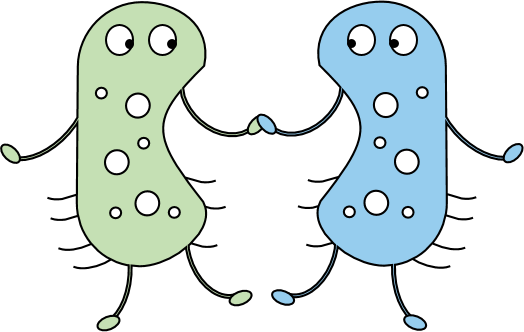
\includegraphics[width=\textwidth]{figures/context/synergy.png}
		}
		\end{center}
	\end{column}
	\begin{column}{.4\textwidth}
	\visible<2->{
			\begin{center}
			Presence of $P_1$ :
			\medskip
			\begin{itemize}
				\item $P_2$'s growth
				\item $P_2$'s severity
				\item $P_2$'s infection duration
			\end{itemize}
			\end{center}
	}
	\end{column}
	\begin{column}{.3\textwidth}
		\begin{center}
		\visible<6>{
		\head{Antagonistic interaction}\\
		}
		\medskip
		\visible<5->{
		$\leftarrow$ decreases\\
		}
		\medskip
		\visible<6>{
		
\includegraphics[width=\textwidth]{figures/context/antagonist.png}
		}
		\end{center}
	\end{column}
	\end{columns}
}


\sframe{Influenza $\rightarrow$ pneumococcus interaction}{
	Often suggested in the literature\\
	\refs{Bosch}{2013}{,} \refs{Mina}{2014}{,} \refs{Opatowski}{2018}{}
	
	\bigskip
	\begin{block}{First evidence: 1918 influenza pandemic}
		\begin{itemize}
			\item Majority of deaths caused by secondary bacterial infections
			\begin{itemize}
				\item \textit{Streptococcus pneumoniae}, \textit{Staphylococcus aureus}, \textit{Haemophilus influenzae}
			\end{itemize}
		\end{itemize}
		\begin{flushright}
		\refs{Brundage}{2008}{, }\refs{Morens}{2008}{, }\refs{Joseph}{2013}{}
		\hspace{-.5cm}
		\end{flushright}
	\end{block}
}



\subsection{Problématique et objectifs de la thèse}

\sframe{Objectives}{
	\begin{itemize}[<+->]
		\item Explore, through modelling, the impact of interactions at the individual scale on infection dynamics at the population scale
		\begin{flushright}
		
\includegraphics[scale=.05]{figures/illustrations/undraw_connecting_teams3_1pgn.png}
		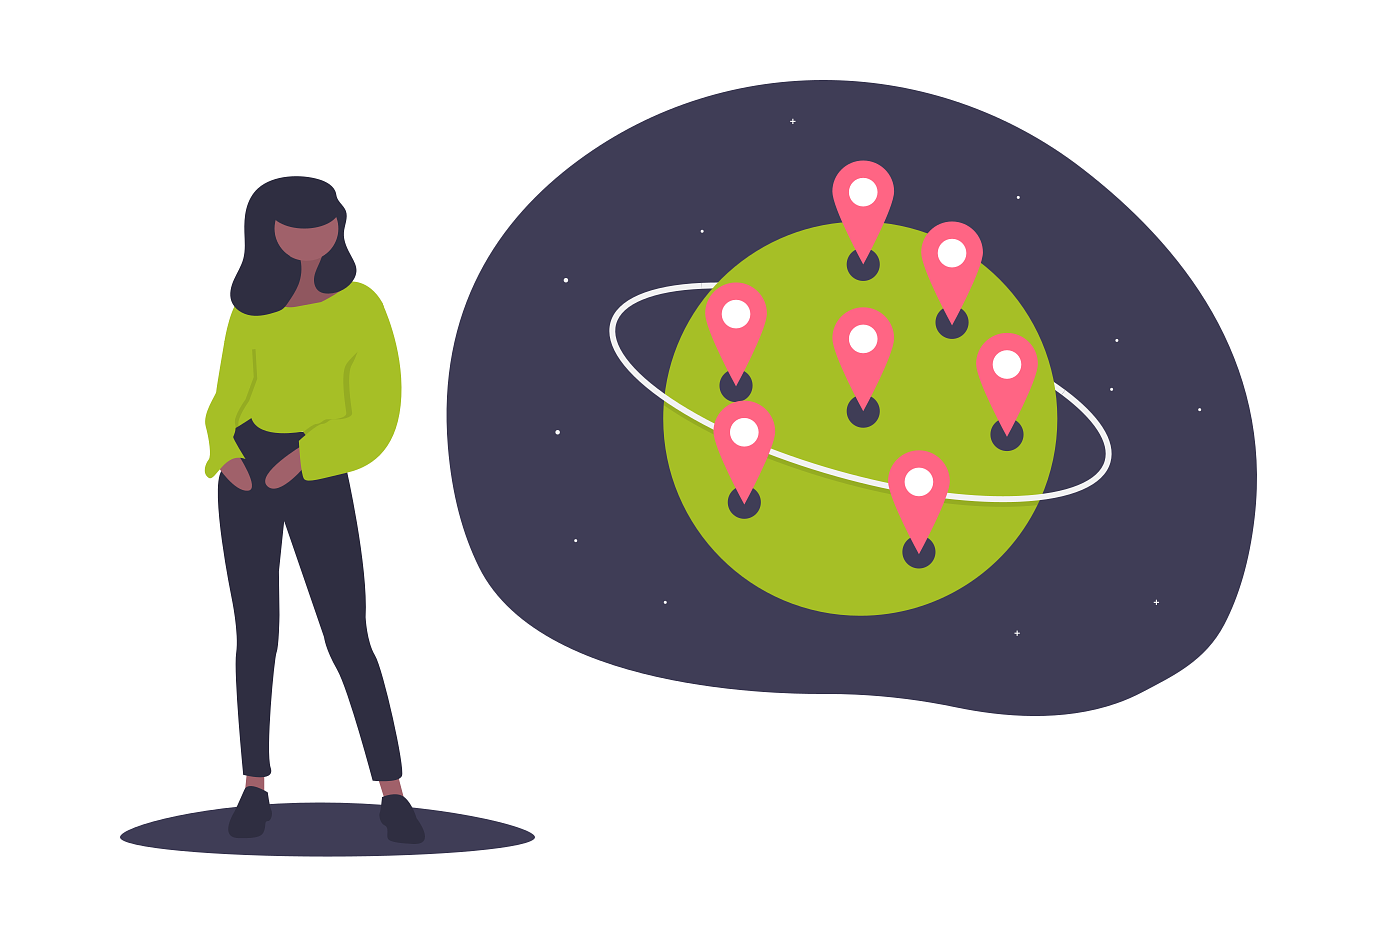
\includegraphics[scale=.05]{figures/illustrations/undraw_around_the_world_v9nu.png}
		\end{flushright}
		\bigskip
		\item Assess, through a simulation study, the ability of several methods to detect an interaction from ecological data
		\begin{center}
		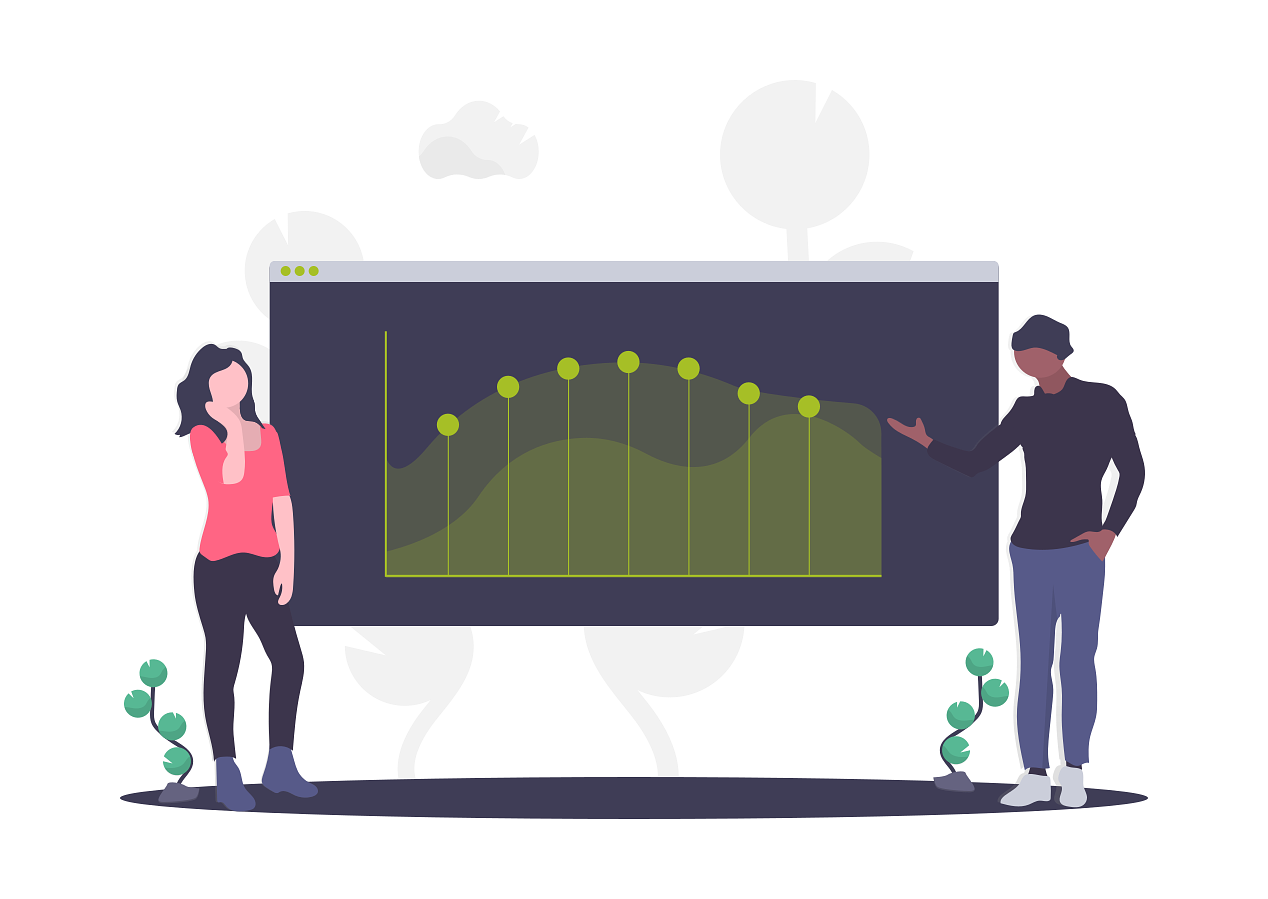
\includegraphics[scale=.07]{figures/illustrations/undraw_growth_analytics_8btt.png}
		\end{center}
	\end{itemize}
}